%\tableofcontents

\section{Introduction}
%motivation
It is long known (since the early 19th~century) that variations in the solar wind evoke disturbances in the magnetosphere \citep{Bartels1962}. Especially strong disturbances, called geomagnetic storms, can be provoked by coronal mass ejections (CMEs), which are embedded within the solar wind. The causes of the strongest geomagnetic storms are the compression of the solar wind magnetic field lines within the CME shock front and the in CMEs enclosed magnetic clouds with their enhanced field strenghts \citep{Bothmer1993}.

These strong geomagnetic disturbances are a threat to sensitive technical systems and exposed humans. Therefore it is important to know when magnetospheric disturbances will occur and how large they will be.\\

%aim
The goal of this paper is to estimate the magnetospheric impact of solar wind in general and to predict it for CMEs in particular.\\


%outline of structure
First we determine the magnitudes of the long-time \Kp{} changes due to solar activity (Sect.~...) and second we measure the extent of seasonal variations stemming from the Earth's orbit (Sect.~...).\\

%general solar wind nowcast
In situ measurements of solar wind are made almost continuously (e.g., at the first Lagrange point (L1)) in front of the magnetosphere. Since 1963 several spacecraft collected more than 50~years of data. The latest spacecraft, e.g., Wind, ACE and DSCOVR (launched in early 2015), provide real-time solar wind data.\footnote{Wind: \url{https://pwg.gsfc.nasa.gov/windnrt/}} \footnote{ACE: \url{http://www.swpc.noaa.gov/products/ace-real-time-solar-wind}} \footnote{DSCOVR: \url{http://www.swpc.noaa.gov/products/real-time-solar-wind}}

This real-time data can be used to estimate various solar wind effects, e.g., the position of the magnetospheric bow shock in front of the Earth, the magnitude of geomagnetic disturbances (\Kp~index), the positions of the polar auroral ovals, the variation of the total electron content (TEC) of the ionosphere, the positional error of global navigation satellite systems (GNSS),...\\

The equatorward auroral boundary position correlates with the \Kp~index.\\

The total electron content (TEC) of the ionosphere has influence on global navigation satellite systems (GNSS). A part of their positional error scales directly with the TEC (in extreme cases up to about \SI{30}{\m}).\\

%CME velocity forecast
The velocity and direction of CMEs can be determined in their early near-Sun stages via remote tracking with coronagraph white-light observations. Using these parameters as input for propagation models, their possible arrival time and arrival velocity at Earth can be derived.\\

%stream velocity forecast from CHs
As coronal holes are the origin of the fast solar wind, their area on the solar disk, seen in EUV images, correlates with the measured velocity of solar wind streams \citep{Vrsnak2007}. This is used to predict the Earth arrival velocity of solar wind streams about 4~days in advance \citep{Rotter2012}.\footnote{\url{http://swe.uni-graz.at/index.php/services/solar-wind-forecast}}\\

With our results presented here we elaborate the step from the predicted CME and stream velocities to the forecast of the possible impact strength on the Earth's magnetosphere.\\

%differences to existing studies
[\citet{Elliott2013}: The \Kp~index and solar wind speed relationship: Insights for improving space weather forecasts]\\

We make an empirical correlation of the solar wind speed with the geomagnetic \Kp~index to obtain the capability to forecast \Kp{} values solely based on the predicted CME and stream velocities.\\

The used OMNI data set consists of minutely data in the time range 1981-01-01 to 2016-12-31.\\

The derived functional dependencies can be used to nowcast/forecast the \Kp~index.\\


%motivation
why use the \Kp{} index?\\


\section{Long-term variations of the \Kp{}~index}

\subsection{\Kp{} data}
The \Kp{} data is obtained from the GFZ~Potsdam\footnote{\url{http://www.gfz-potsdam.de/de/kp-index/}}, where the index is now maintained. The data used in this analysis covers the time period 1932--2016.\\

The \Kp{} frequency distribution for the time period 1932--2016 shows that the highest frequencies occur around low \Kp{} values of 1+ and to higher \Kp{} values the frequencies seem to decline exponentially (see Fig.~\ref{fig:Kp_histogram}). A \Kp{} value of 9o occurred only 29 times in this time interval.\\
\begin{figure}
	\fcapside[\FBwidth]{
		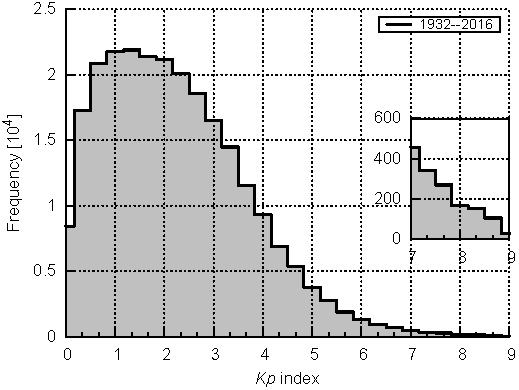
\includegraphics[width=0.5\textwidth]{chapter2/figures/Kp_histogram.pdf}
	}{
		\caption{\Kp{} frequency distribution for the time period 1932--2016. \Kp{} data from the GFZ~Potsdam.}
		\label{fig:Kp_histogram}
	}
\end{figure}

\subsection{\Kp{} variations with solar activity}
solar activity is tracked with the sunspot number (SSN); SSN data\\
The general \Kp{} distribution, seen before in Fig.~\ref{fig:Kp_histogram}, averages over solar activity. With different states of solar activity the \Kp{} frequency distributions' shape varies. This can be seen from the yearly distributions, sorted and colored by yearly SSN (see Fig.~\ref{fig:Kp_histogram_yearlySSN}). The distribution's peak position scales with SSN, that is, a high yearly SSN results also in more large \Kp{} values.\\
\begin{figure}
	\fcapside[\FBwidth]{
		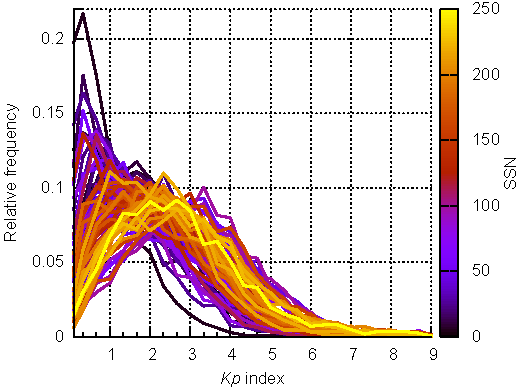
\includegraphics[width=0.5\textwidth]{chapter2/figures/Kp_histogram_yearlySSN.pdf}
	}{
		\caption{Yearly \Kp{} frequency distributions of the period 1932--2016 sorted and colored by SSN. \Kp{} data from the GFZ~Potsdam and the yearly SSN from the SILSO World Data Center.}
		\label{fig:Kp_histogram_yearlySSN}
	}
\end{figure}

The time series of yearly average \Kp{} values in the time span 1932--2016 shows an imprint of the solar cycles (see the top graphs in Fig.~\ref{fig:yearly_kp-ssn_correlation_c}).
\begin{figure}
	\fcapside[\FBwidth]{
		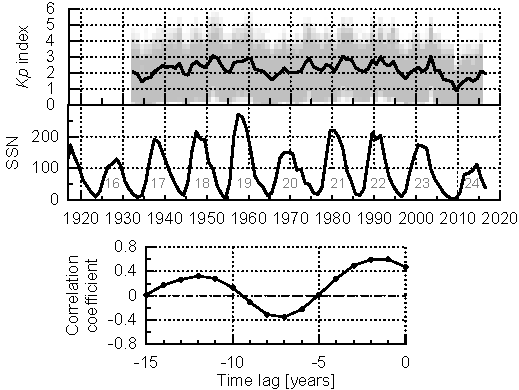
\includegraphics[width=0.5\textwidth]{chapter2/figures/yearly_kp-ssn_correlation_c.pdf}
	}{
		\caption{Yearly \Kp~index from GFZ~Potsdam and yearly SSN from the SILSO World Data Center (1932--2016) with cycle number (top). The correlation coefficients with the yearly SSN are calculated for time lags back to -15~years (bottom).}
		\label{fig:yearly_kp-ssn_correlation_c}
	}
\end{figure}
The \Kp{} pattern follows the solar cycle minima and maxima as well as the changes in magnitude between solar cycles. The yearly mean \Kp{} shifts about 1~unit for both variations.

As expected, the \Kp{}~index correlation with solar activity shows an 11-year period (see bottom graph in Fig.~\ref{fig:yearly_kp-ssn_correlation_c}). The highest correlation coefficient 0.60 is found with a time lag of $-1$~year, that is, the yearly average \Kp{} follows the SSN of the previous year.
%Kp-ssn cc: 0.5971

cause are CHs, see paper...\\

The yearly mean \Kp~indices with respect to the 1-year lagged SSN show a raise in \Kp{} with increasing SSN, which is seen in Fig.~\ref{fig:Kp_SSN_fit_d}.
\begin{figure}
	\fcapside[\FBwidth]{
		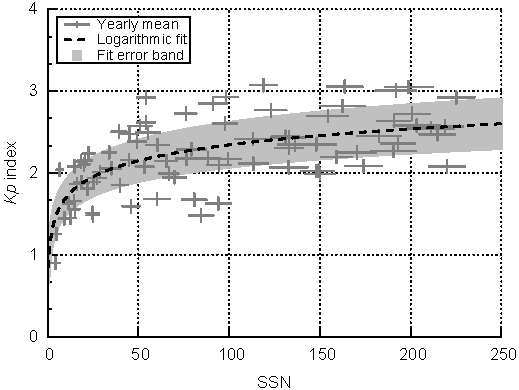
\includegraphics[width=0.5\textwidth]{chapter2/figures/Kp_SSN_fit_d.pdf}
	}{
		\caption{Yearly mean \Kp~index over 1-year lagged SSN (+) with the weighted logarithmic fit (dashed). The error bars denote the SSN standard deviation and the relative weight from the yearly data coverage. The shaded area represents the fit error band derived from the estimated standard deviations of the fit parameters. The function (\ref{eq:log_fit_function}) is used for the weighted fit. The yearly \Kp{} mean values are obtained from GFZ~Potsdam data and the yearly SSN from the SILSO World Data Center.}
		\label{fig:Kp_SSN_fit_d}
	}
\end{figure}

We perform a fit to obtain an analytical relation for this dependency. \Kp{} itself is a quasi-logarithmic index, so it is apparent to use a logarithmic fit function:
\begin{align}
	f(x) = a \cdot \ln(x) + b	\,.	\label{eq:log_fit_function}
\end{align}
The fitted parameter values are $a = 0.281(43)$ and $b = 1.05(19)$ and lead to the relation
\begin{align}
	\Kp(ssn) = 0.28 \cdot \ln(ssn) + 1.1	\,.
\end{align}
% log fit parameters:
% a 0.281126         +/- 0.04267
% b 1.04923          +/- 0.19
In the fit result, plotted in Fig.~\ref{fig:Kp_SSN_fit_d}, the mean \Kp{} is 1.05(19) for a SSN of 1 and 2.53(30) for a SSN of 200. The fit error band has a width of about half a \Kp~unit.\\


\subsection{Seasonal \Kp{} variations}
There also are seasonal variations in the magnetospheric disturbances. Looking at the monthly \Kp{} frequency distributions for different seasons of the year, it is apparent that in the months May--August the \Kp{} peak frequency is higher than in the rest of the year (see Fig.~\ref{fig:Kp_histogram_monthly}). In March/April and September/October the \Kp{} values \num{>3} are more abundant.\\
\begin{figure}
	\fcapside[\FBwidth]{
		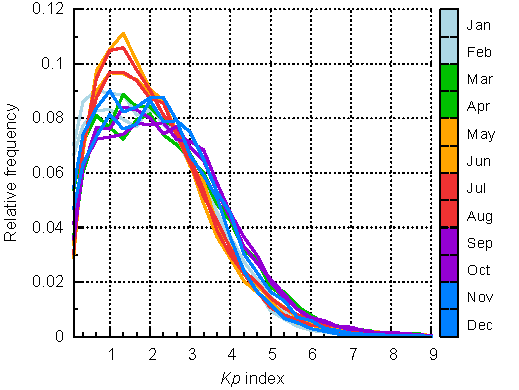
\includegraphics[width=0.5\textwidth]{chapter2/figures/Kp_histogram_monthly.pdf}
	}{
		\caption{Monthly \Kp{} frequency distributions colored by months of the year. \Kp{} data of the time period 1932--2016 from the GFZ~Potsdam.}
		\label{fig:Kp_histogram_monthly}
	}
\end{figure}
These seasonal \Kp{} changes arise from seasonal variations of the solar wind parameters at Earth, which stem from Earth's yearly changes in orbital distance and heliographic latitude (as discussed in Sect.~XX of MVVB-Paper). Another seasonal effect comes from the Earth's rotation axis tilt (\SI{+-23.44}{\degree}) (obliquity to the ecliptic), which changes the direction of the Earth's magnetic dipole axis to the Sun over the year (see bottom panel of Fig.~\ref{fig:Kp_seasonal}). The rate of magnetic reconnection between solar wind and magnetosphere depends on both fields' direction to each other (parallel/antiparallel) (see Figure in Basics...).\\

\Kp{} seasonal variation effects from seasonal changing Sun tilt, Earth tilt and Earth distance.\\
causes (see citet{Rangarajan1997} p.~1282 and mention Bartels1963 too):\\
- Earth's rotation axis tilt (\SI{+-23.44}{\degree}) (obliquity to orbit/inclination of equator)\\
- solar rotation axis tilt (\SI{+-7.25}{\degree}) (cite 'NASA Earth fact sheet')\\
- Earth's varying solar distance of \SI{+-1.67}{\percent}\\
read Bothmer1998 Ch 3...\\


We quantify the magnitude of these effects. \Kp{} frequency distributions by month, see Fig.~\ref{fig:Kp_seasonal}.\\
\begin{figure}
	\fcapside[\FBwidth]{
		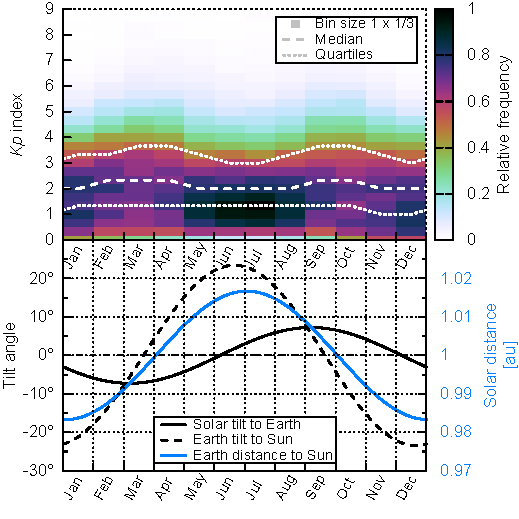
\includegraphics[width=0.5\textwidth]{chapter2/figures/Kp_seasonal.pdf}
	}{
		\caption{\Kp{} frequency distributions by month for the time period 1932--2016 with median and quartile values (top). Solar tilt angle to Earth, Earth tilt angle to Sun and Earth distance to Sun are approximated with trigonometric fuctions (bottom). switch panels...}
		\label{fig:Kp_seasonal}
	}
\end{figure}
for high \Kp{} values (>~4?) there are yearly frequency maxima at the equinoxes and minima at the solstices. this variation amounts to more than 1?~\Kp~unit...\\

The magnitudes of the SSN variation $\Kp(ssn)$ and the seasonal variation \Kp(month) are of a similar order...?\\

Both variations are an indirect influence through solar wind (see paper).\\


\section{\Kp{} nowcast from in situ solar wind measurements}

\subsection{Solar wind-magnetosphere coupling}
%literature
The coupling between the solar wind and the magnetosphere is governed by reconnection and compression of the magnetic field lines (see Basics...).\\

the dayside reconnection is asymmetric\\

To describe this, some coupling functions with different complexity were proposed (Newell, cites? and list).\\

dayside reconnection:\\
``$E_\text{y}$ is the rate at which southward magnetic flux is convected to the magnetosphere by the solar wind ($-v_\text{x} \cdot B_\text{z}$) in GSM coordinates,'' \citep{Russell2007}\\

the product of the proton velocity $v$ and the magnetic field z-component in geocentric solar magnetospheric (GSM) coordinates $B_\text{z}$:
\begin{align}
	?check vectors  E_\text{y} = -v_\text{x} \times B_\text{z}\,\text{(GSM)}	\label{eq:coupling_vxB}
\end{align}
If not specified otherwise, $B_\text{z}$ is always meant to be in GSM coordinates hereafter.\\

argue for \vBz:\\
- 3hmin(\vBz) performs in rank correlation slightly better than the sophisticated Newell formula. really?\\
- simple to calculate\\
- ...\\

We settle for \vBz{} as the coupling function to analyze.\\

It also is known that the solar wind velocity itself already correlates strongly with the \Kp~index. In fact \citet{Machol2013} even proposed a linear function of the \Kp~index as a best proxy for corrupted real-time velocity measurements made by the Advanced Composition Explorer (ACE) spacecraft.\\

\subsection{Data set, data processing and correlation}
\label{sec:data_set__data_processing_and_correlation}
%determine data basis
The \Kp{} time series started in 1932 when there were no spacecraft to measure in situ solar wind. Thus, the surveyed time range is defined by the available in situ solar wind data. The OMNI data set collects the longest continuous solar wind measurements at \SI{1}{\au},
it covers hourly data since 1963; 5-minute and minutely data since 1981.\\

why this data set? - because of long time coverage, to magnetospheric bow shock calculated solar wind and integrated geomagnetic indices (see Paper...)\\

%argue for averaging method
The \Kp{}~index represents maximal variations within 3-hour time intervals. Any solar wind parameter that will be correlated with it also has to have the same time resolution. Additionally to adapting the time resolution, we have to consider by which means it should be done. Simple 3-hour average values should have a lower correlation coefficient than the solar wind parameter's 3-hourly maximal variation.\\

%argue for high resolution, deliberate between hourly and minutely data
The 3-hour maximal variations are obviously higher when using high resolution data. Thus, to be able to correlate \Kp{} with solar wind data, high resolution data (e.g., 1~min) is needed to determine the maximal solar wind variations within each 3-hour interval.\\

%compare data sets (hourly/minutely->what is good for 3hmax?\\
The longest time coverage has the hourly OMNI data set (since 1963), however we prefer to use the minutely OMNI data with the time range 1981--2016, to benefit from higer correlation coefficients (see Figs?).\\

% Velocity-\Kp{} correlation coefficients for maximum, mean and minimum, see Fig.~\ref{fig:cc_lag_data_b}.\\
% \begin{figure}
% 	\resizebox{\hsize}{!}{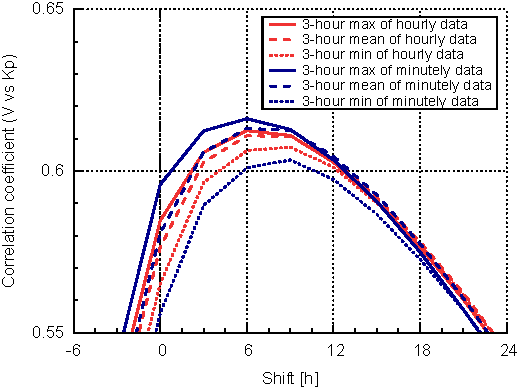
\includegraphics{chapter2/figures/cc_lag_data_b.pdf}}
% 	\caption{Velocity-\Kp{} correlation coefficients for different time shifts. Hourly and minutely OMNI data from 1981--2016 with max, mean and min averaging.}
% 		\label{fig:cc_lag_data_b}
%	}
% \end{figure}
% 3-hour max data has a higher correlation coefficient than 3-hour mean data. Max averaging achieves highest cc.\\
% hourly data has slightly lower cc's than minutely data. Why? mean of mean is mean.\\

Pearson correlation coefficients; use Spearman rank instead?\\
correlate positive and negative values separately?\\

\Kp{}-\vBz{} Pearson correlation coefficients for mean and minimum, see Fig.~\ref{fig:cc_lag_data_d_KpvsVBzgsm}.\\
\begin{figure}
	\fcapside[\FBwidth]{
		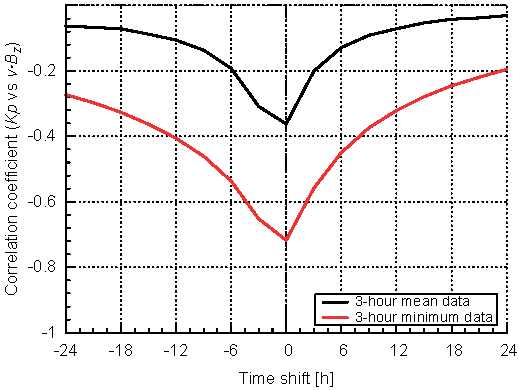
\includegraphics[width=0.5\textwidth]{chapter2/figures/cc_lag_data_d_KpvsVBzgsm.pdf}
	}{
		\caption{\Kp-\vBz{} correlation coefficients for different time shifts. Minutely OMNI data from 1981--2016 processed with mean (black) and minimum (red) 3-hour averaging.}
		\label{fig:cc_lag_data_d_KpvsVBzgsm}
	}
\end{figure}
%highest correlation coefficients:
%min:	0.00000    -0.717240
%mean:	0.00000    -0.362237
%max:	0.00000     0.293137
The largest correlation is found for the 3-hour minimum data without time shift. It is a negative correlation with a coefficient of $-0.72$.\\

We use \vBz{} 3-hour minimum values, as a result their frequency distribution and its peak is asymmetrically shifted to negative values, as seen in Fig.~\ref{fig:histogram_VBzgsm}.\\
\begin{figure}
	\fcapside[\FBwidth]{
		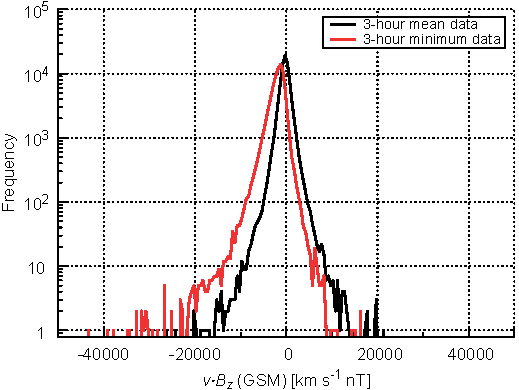
\includegraphics[width=0.5\textwidth]{chapter2/figures/histogram_VBzgsm.pdf}
	}{
		\caption{Frequency distributions of \vBz{} for 3-hour mean (black) and minimum (red) minutely OMNI data from 1981--2016.}
		\label{fig:histogram_VBzgsm}
	}
\end{figure}
%vBz frequency shifts:
% min shift: -1250
% mean shift: -250
% max shift: -750
even the 3-hour mean shows a slight offset in position (why?)\\


\subsection{Functional dependency}
%distribution
The frequency distribution over the \Kp-\vBz{} space is shaped like a candle flame inclined to negative values by a light breeze, see top panel in Fig.~\ref{fig:Kp_2dhistogram_VBzgsm_sws_d}.
\begin{figure}
	\fcapside[\FBwidth]{
		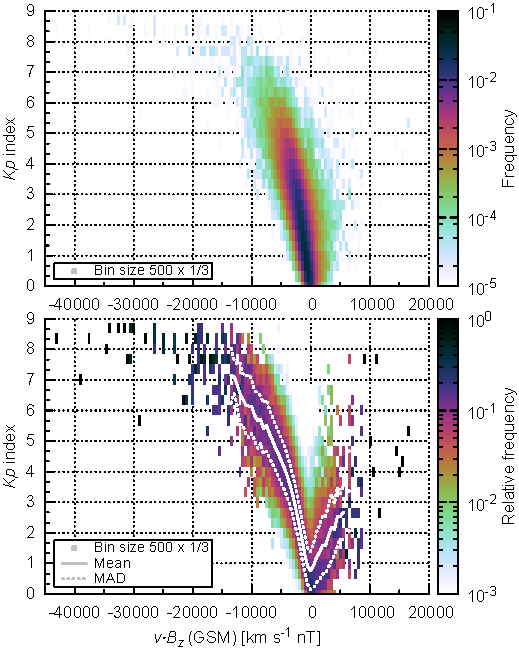
\includegraphics[width=0.5\textwidth]{chapter2/figures/Kp_2dhistogram_VBzgsm_sws_d.pdf}
	}{
		\caption{\Kp{} versus \vBz{} frequency distribution (top) and its relative distribution (bottom) with the mean \Kp{} values (solid) and their mean absolute deviation (dotted). It is 3-hour minimum data from the minutely OMNI data set (1981--2016). The bin size is \SI{500}{\km\per\s\nano\tesla} and \SI{1/3}{\Kp~unit} respectively.}
		\label{fig:Kp_2dhistogram_VBzgsm_sws_d}
	}
\end{figure}

%dependency
To determine a functional dependency we look at the relative frequencies per \vBz-interval and their mean \Kp{} values, which are plotted in the bottom panel of Fig.~\ref{fig:Kp_2dhistogram_VBzgsm_sws_d}. The mean absolute deviation (MAD) of the mean has a mean size of \SI{0.7}{\Kp~units}. This probability distribution is asymmetrically V-shaped around zero, having a larger and steeper negative arm. This effect is not a result of the data reducing method (3-hour minimum), because for 3-hour mean data the asymmetry also exists (fig...?). Rather the steeper negative arm is a consequence of the half-wave rectifier coupling of the solar wind magnetic field direction to the magnetosphere as described in Sect~(coupling section...).\\
%MAD: 2.211/3 = 0.737 Kp units

%determine fitting functions
Since the \Kp~index has a quasi-logarithmic scaling (see Basics...), a logarithmic function is the obvious choice as a fit function. Furthermore, the depending argument consists of a product of two solar wind parameters which individually scale logarithmically with \Kp{}. These reasons are why we use the logarithm of a parabola for the fitting approach:
\begin{align}
	f(x) &= \ln(x^2)	\,.	\label{eq:log_square_function}
\end{align}
We introduce a horizontal shifting parameter $x2$ because the distribution's center is slightly offset. To be able to replicate the asymmetry in both arms, we split the fit function into a negative and a positive part:
\begin{align}
	f(x) &=
	\begin{cases}
		\,f_-(x) &\text{for } x < 0	\,,\\
		\,f_+(x) &\text{for } x \ge 0	\,.
	\end{cases}	\label{eq:log_square_fit_function}
\end{align}
This way both arms can be scaled individually with the scaling factors for the negative and positive parts $a$ and $c$. The resulting logarithmic fit functions are
\begin{align}
	f_-(x) &= a \cdot \ln((x + x2)^2 + d) + b	\,,\\
	f_+(x) &= c \cdot (f_-(x) - f_-(-x2)) + f_-(-x2)	\,,
\end{align}
with the vertical shifting parameter $b$ and the depth parameter $d$.\\

The resulting fit is plotted in Fig.~\ref{fig:Kp_2dhistogram_VBzgsm_sws_fit_e} with the fit coefficients $a = 1.258(19)$, $b = -17.04(33)$, $c = 0.467(20)$, $d = \num{1.416(68)e6}$ and $x2 = 163(20)$ for units of [\si{\km\per\s \nano\tesla}].\\
%high precision values:
% a = 1.25788(0.019)\\
% b = -17.0394(0.33)\\
% c = 0.467039(0.0197)\\
% d = 1.41639e6(0.067795e6)\\
% x2 = 162.907(20.642)\\
\begin{figure}
	\fcapside[\FBwidth]{
		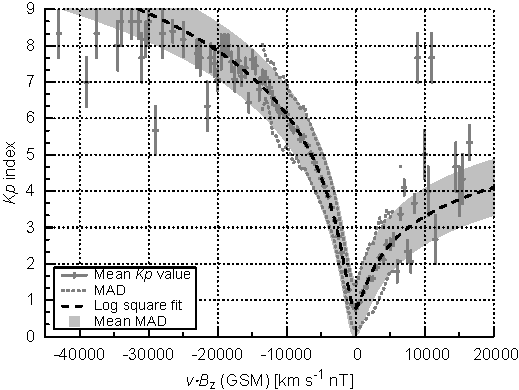
\includegraphics[width=0.5\textwidth]{chapter2/figures/Kp_2dhistogram_VBzgsm_sws_fit_e.pdf}
	}{
		\caption{Mean \Kp{} values (+) and MAD values (dotted) per \vBz~interval. The error bars represent the relative data count. The logarithmic fit (dashed) is plotted with a mean MAD band (shaded area). The splitted function (\ref{eq:log_square_fit_function}) is used for the weighted fit. OMNI data from the time period 1981--2016 is used.}
		\label{fig:Kp_2dhistogram_VBzgsm_sws_fit_e}
	}
\end{figure}

Thus, the solar wind dependency relation condenses to:
\begin{align}
	\text{\Kp}_-(vB_\text{z}) &= 1.26 \cdot \ln((vB_\text{z} + 160)^2 + \num{1.42e6}) - 17.0	\,,	\label{eq:kpvsvbz_dependency_function_negative}\\
	\text{\Kp}_+(vB_\text{z}) &= 0.47 \cdot (\text{\Kp}_-(vB_\text{z}) - \text{\Kp}_-(-160)) + \text{\Kp}_-(-160)	\,.	\label{eq:kpvsvbz_dependency_function_positive}
\end{align}
This relation can be used together with real-time in situ measurements from spacecraft located at L1 to nowcast the actual \Kp~index.\\


\section{\Kp{} forecast from remote CME observations}
Compared to the steady solar wind, which can be measured reliably only from in situ measurements, CMEs can already be sighted raising from their source region on the solar surface. From remote coronagraph observations some CME properties can be estimated and modeled to Earth, like its propagation direction and its arrival time and velocity (cites...). Thus, early observations enable a heads-up time only depending on the CME's propagation speed to Earth. This travel duration can be more than 4~days for slow events with average solar wind speeds, about 40~hours for fast events with average speeds of \SI{1000}{\km\per\s} and down to 20~hours and even below for the rare extreme cases, e.g., 19~hours for the event observed by \citet{Carrington1859} on 1~September 1859 and about 21~hours for the event on 23~July 2012 \citep{Russell2013,Temmer2015}.\\

To make use of the heads-up time for CMEs, we simplify the coupling relation from before (\ref{eq:coupling_vxB}) by neglecting its magnetic field part, which cannot be determined from remote observations. Only the solar wind velocity is left as a coupling parameter.\\

\subsection{CME velocity estimation}
methods and modeling...?\\
GCS, CAD modeling -> propagation direction and apex height-time profile -> acceleration and velocity kinematics...\\
-> example event CME?\\

\subsection{SWS CME list}
For the following analysis we use the list of solar wind structures (SWS) created and updated by \citet{Richardson2000,Richardson2012}, who characterized the near-Earth solar wind structures since 1963. All periods related to ICMEs in the OMNI solar wind data set were identified and flagged.\\

The SWS list for 1963--2016 was kindly provided by Ian~Richardson (private communication).\\

SWS list for 1963--2015 by \citep{Richardson2000,Richardson2012} is available via registration at CEDARweb\footnote{CEDARweb website for Solar Wind Structures: \url{http://cedarweb.vsp.ucar.edu/wiki/index.php/Tools_and_Models:Solar_Wind_Structures} (existent in 2017-10-29)}.\\
List of near-Earth ICMEs since January 1996 by \citet{Cane2003,Richardson2010}. Available as ACE Level~3 data for the period 1995--mid2016\footnote{ACE Level~3 data website -- list of near-Earth ICMEs: \url{http://www.srl.caltech.edu/ACE/ASC/DATA/level3/icmetable2.htm} (existent in 2017-10-29)}.\\

The CME fraction of the OMNI time series for the period 1981--2016 is \SI{15.8}{\%} (5.53~years) and that for the period 1963--2016 is \SI{17.0}{\%} (9.01~years).\\

% acknowledgments:\\
% The hourly solar wind structure list was kindly provided by Ian~Richardson of the NASA Goddard Space Flight Center and CRESST/University of Maryland via the CEDAR Database at the National Center for Atmospheric Research, which is supported by the National Science Foundation.\\


\subsection{Data processing and correlation}
Again we calculate 3-hour extreme values using the minutely OMNI data to profit from higher correlation coefficients, like done for the data processing of the \vBz{} analysis in Sect.~\ref{sec:data_set__data_processing_and_correlation}. For the velocity these are 3-hour maximum values. The comparison between the 3-hour maximum and the 3-hour mean frequency distributions show that their mean position raises from 405 to \SI{425}{\km\per\s}, see Fig.~\ref{fig:histogram_V_b}.\\
%the SWS1 mean raises from 435 to 455~km/s in 3hmax data...\\
\begin{figure}
	\fcapside[\FBwidth]{
		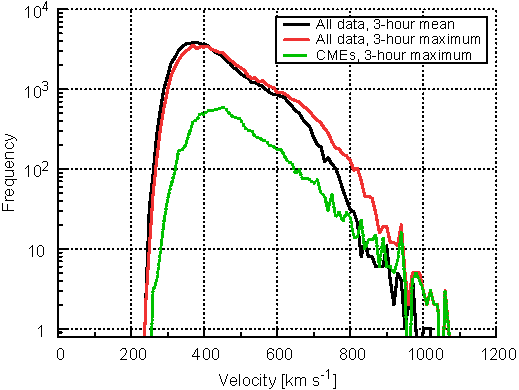
\includegraphics[width=0.5\textwidth]{chapter2/figures/histogram_V_b.pdf}
	}{
		\caption{Solar wind velocity frequency distributions for 3-hour mean (black), maximum (red) and maximum of the CME part (green). Minutely OMNI data from the period 1981--2016 is used.}
		\label{fig:histogram_V_b}
	}
\end{figure}

Using the CME periods from the SWS list as a filter, the CME part and non-CME part of the data can be examined separately. Their frequency distributions show that in faster solar wind the CME share is rising until eventually in the region above about \SI{900}{\km\per\s} there exist only CMEs, see Fig.~\ref{fig:histogram_V_b}.

The CME part of the data is correlated with the \Kp~index independently from the remaining solar wind, see Fig.~\ref{fig:cc_lag_sws_d}.
\begin{figure}
	\fcapside[\FBwidth]{
		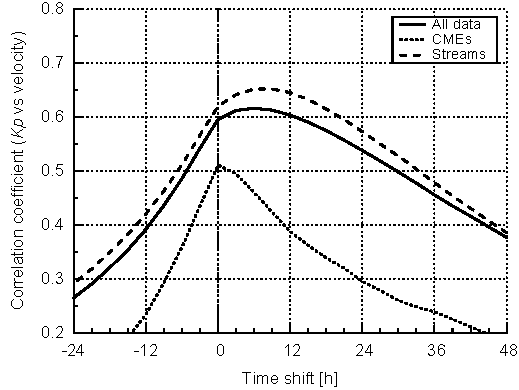
\includegraphics[width=0.5\textwidth]{chapter2/figures/cc_lag_sws_d.pdf}
	}{
		\caption{\Kp{}-velocity correlation coefficients for different time shifts. The correlations for the whole solar wind data (solid), for solar wind without CMEs (dashed) and for CMEs only (dotted) are plotted. The used data is the 3-hour maximum of the minutely high resolution OMNI data.}
		\label{fig:cc_lag_sws_d}
	}
\end{figure}
The correlation for CME related data is smaller than that for the regular solar wind. Its maximal correlation coefficient with a value of 0.51 is without time shift, see Table~\ref{tab:correlation_coefficients_kpvsv}.
\begin{table*}
	\caption{Time lags with the highest correlation coefficients for the \Kp{}-velocity relation. The used data is the 3-hour maximum of the minutely high resolution OMNI data.}
	\label{tab:correlation_coefficients_kpvsv}
	\centering
	\begin{tabular}{lcc}
		\hline\hline
		Data	&Time lag [hours]	&Correlation coefficient\\
		\hline
		All data	&6	&0.622\\
		w/o CMEs	&9	&0.661\\
		CMEs	&0	&0.511\\
		\hline
	\end{tabular}
\end{table*}
% the best lag times are:\\
% sws: +6 h\\
% sws1: 0 h\\
% sws23: +9 h\\
% 
% correlation coefficients\\
% SWS1\\
% 0	0.511093\\
% SWS23\\
% lag	cross	auto x	auto y\\
% -3	0.660694\\
% 0	0.620113\\
% SWS\\
% lag	cross	auto x	auto y\\
% -2	0.621539\\
% 0	0.595784\\
The regular solar wind without CMEs shows a higher correlation with \Kp{} and its maximal coefficient of 0.66 is at a positive time shift of 9~hours, that is, the \Kp~index forecasts the velocity of regular solar wind 9~hours in advance.

The positive time shift can be explained with the occurence of interaction regions followed by high speed streams (HSS). When a slow solar wind stream is followed by a fast one, the compression at their interface leads to enhanced solar wind densities and magnetic field strengths. The peak velocity of a HSS naturally appears after the interaction region. Therefore the \Kp-impact of the enhanced magnetic field is correlated with the higher velocity of the HSS, yielding the observed positive time shift.\\


\subsection{Functional dependency for CMEs}
The general \Kp-velocity dependency is apparent in the tilt of its distribution, see top panel of Fig.~\ref{fig:Kp_2dhistogram_V_sws_c}.
\begin{figure}
	\fcapside[\FBwidth]{
		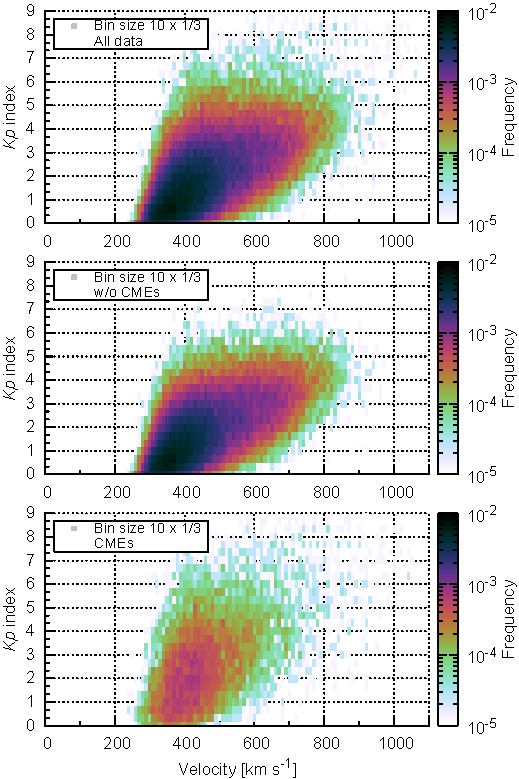
\includegraphics[width=0.5\textwidth]{chapter2/figures/Kp_2dhistogram_V_sws_c.pdf}
	}{
		\caption{\Kp-velocity distributions for the whole solar wind data, for solar wind without CMEs and for CMEs only. The used data is the 3-hour maximum of the minutely high resolution OMNI data. For the CME separation the SWS list from \citet{Richardson2012} is used. The bin size is \SI{10}{\km\per\s} and \SI{1/3}{\Kp~unit} respectively.}
		\label{fig:Kp_2dhistogram_V_sws_c}
	}
\end{figure}
The comparison with the CME data shows that \Kp{} values \num{>7} and velocities \SI{>900}{\km\per\s} are almost always associated with CME related periods, see middle and bottom panel of Fig.~\ref{fig:Kp_2dhistogram_V_sws_c}.\\

To find a functional dependency for the mean \Kp{} value we look at the relative frequencies per velocity interval, which are plotted in the bottom panel of Fig.~\ref{fig:Kp_2dhistogram_V_sws1_c}.
\begin{figure}
	\fcapside[\FBwidth]{
		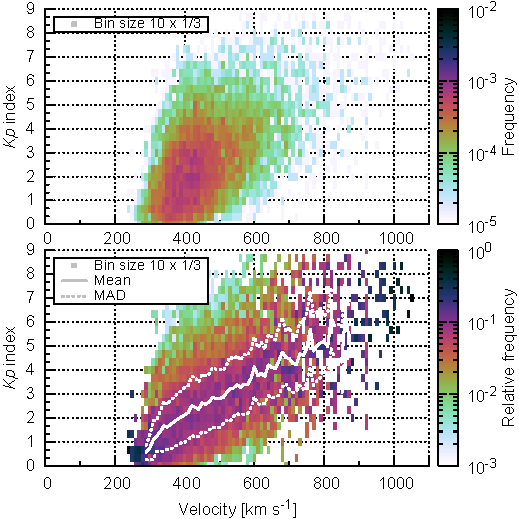
\includegraphics[width=0.5\textwidth]{chapter2/figures/Kp_2dhistogram_V_sws1_c.pdf}
	}{
		\caption{CME part of the \Kp-velocity distribution (same as third panel of Fig.~\ref{fig:Kp_2dhistogram_V_sws_c}) and its relative distribution per velocity interval with the mean \Kp{} values (solid) and their mean absolute deviation (dotted). The bin size is \SI{10}{\km\per\s} and \SI{1/3}{\Kp~unit} respectively.}
		\label{fig:Kp_2dhistogram_V_sws1_c}
	}
\end{figure}
The mean \Kp{} value seems to scale almost linear with the solar wind velocity. The mean absolute deviation of the mean has a mean size of about \SI{1.1}{\Kp~units}.\\
%MAD: 3.338/3 = 1.113 Kp units

%determine fitting function
Again, as the \Kp~index has a quasi-logarithmic scaling, a logarithmic function is the obvious choice for the fitting process, for which thus the logarithmic function
\begin{align}
	f(x) = a \cdot \ln(x + x1) + b	\label{eq:log_offset_fit_function}
\end{align}
is used, with the scaling factor $a$, the location parameter $x1$ and the vertical shifting parameter $b$.\\

The resulting fit is plotted in Fig.~\ref{fig:Kp_2dhistogram_V_sws1_fit_e}, with velocity in units of [\si{\km\per\s}] its parameters are $a = \num{10.6(34)}$, $b = \num{-73(28)}$ and $x1 = \num{8.1(43)e2}$.\\
%10.6075 (3.4)\\
%-73.1694 (28.)\\
%806.943 (430)\\
\begin{figure}
	\fcapside[\FBwidth]{
		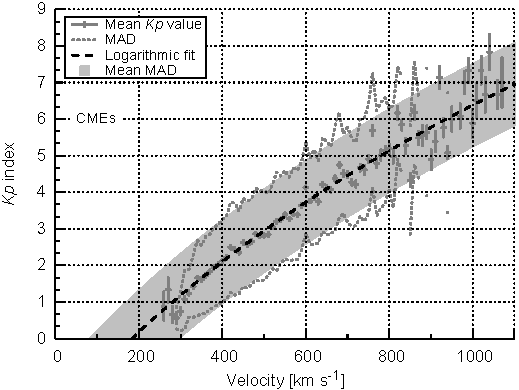
\includegraphics[width=0.5\textwidth]{chapter2/figures/Kp_2dhistogram_V_sws1_fit_e.pdf}
	}{
		\caption{Mean \Kp{} values (+) and MAD values (dotted) per velocity interval for the CME part of the data. The error bars represent the relative data count. The logarithmic fit (dashed) is plotted with a mean MAD band (shaded area). The function (\ref{eq:log_offset_fit_function}) is used for the weighted fit. The CME part of the OMNI data from the period 1981--2016 is obtained using the SWS list from \citet{Richardson2012}.}
		\label{fig:Kp_2dhistogram_V_sws1_fit_e}
	}
\end{figure}
This leads to the CME dependency function
\begin{align}
	\Kp(v) = 11 \cdot \ln(v + 800) - 70	\,,	\label{eq:kpvsv_dependency_function}
\end{align}
which can be used to forecast the \Kp{}~index from the estimated CME arrival velocity.\\

\subsection{Functional dependency for non-CMEs}

use of by 9-hours shifted data..., see Fig.~\ref{fig:cc_lag_sws_d}\\

To find a functional dependency for the mean \Kp{} value we look at the relative frequencies per velocity interval, which are plotted in the bottom panel of Fig.~\ref{fig:Kp_2dhistogram_V_sws23_c}.
\begin{figure}
	\fcapside[\FBwidth]{
		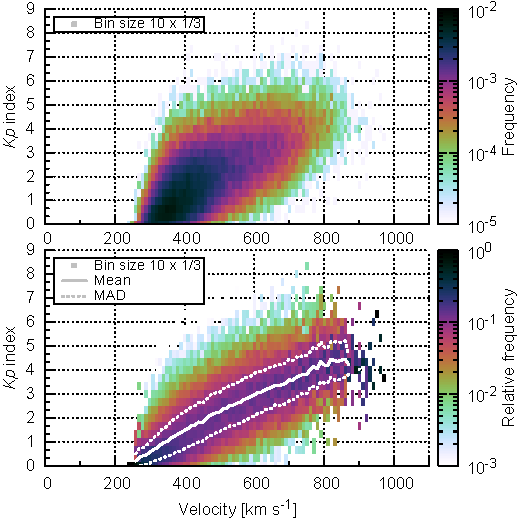
\includegraphics[width=0.5\textwidth]{chapter2/figures/Kp_2dhistogram_V_sws23_c.pdf}
	}{
		\caption{Non-CME part of the \Kp-velocity distribution (similar to second panel of Fig.~\ref{fig:Kp_2dhistogram_V_sws_c}, but with the by 9-hours shifted data) and its relative distribution per velocity interval with the mean \Kp{} values (solid) and their mean absolute deviation (dotted). The bin size is \SI{10}{\km\per\s} and \SI{1/3}{\Kp~unit} respectively.}
		\label{fig:Kp_2dhistogram_V_sws23_c}
	}
\end{figure}
The mean \Kp{} value seems to scale almost linear with the solar wind velocity. The mean absolute deviation of the mean has a mean size of about \SI{0.7}{\Kp~units}.\\
%MAD: 2.226/3 = 0.742 Kp units
%MAD: 2.332/3 = 0.777 Kp units for 300--900km/s
%MAD: 2.389/3 = 0.796 Kp units for 350--900km/s
%MAD: 2.454/3 = 0.818 Kp units for 350--850km/s

%determine fitting function
Again, as the \Kp~index has a quasi-logarithmic scaling, a logarithmic function is the obvious choice for the fitting process, for which thus the logarithmic function (\ref{eq:log_offset_fit_function}) is used.\\

The resulting fit is plotted in Fig.~\ref{fig:Kp_2dhistogram_V_sws23_fit_e} and the fit parameters are $a = \num{5.88(38)}$, $b = \num{-3.70(29)e1}$ and $x1 = \num{2.99(49)e2}$, with velocity in units of [\si{\km\per\s}].\\
%a1 = 5.88(38)
%b1 = -37.0(29)
%x1 = 299(49)
\begin{figure}
	\fcapside[\FBwidth]{
		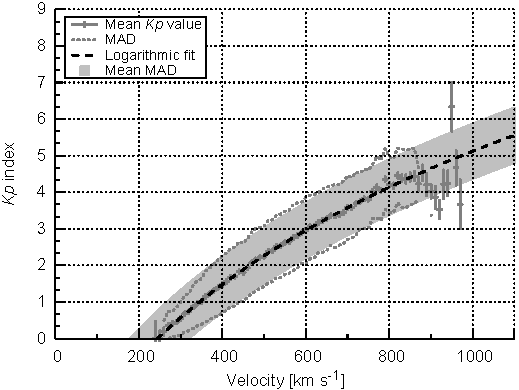
\includegraphics[width=0.5\textwidth]{chapter2/figures/Kp_2dhistogram_V_sws23_fit_e.pdf}
	}{
		\caption{Mean \Kp{} values (+) and MAD values (dotted) per velocity interval for the non-CME part of the data, shifted by 9-hours. The error bars represent the relative data count. The logarithmic fit (dashed) is plotted with a mean MAD band (shaded area). The function (\ref{eq:log_offset_fit_function}) is used for the weighted fit. The non-CME part of the OMNI data from the period 1981--2016 is obtained using the SWS list from \citet{Richardson2012}.}
		\label{fig:Kp_2dhistogram_V_sws23_fit_e}
	}
\end{figure}
This leads to the non-CME dependency function
\begin{align}
	\Kp(v) = 5.9 \cdot \ln(v + 300) - 37	\,,	\label{eq:kpvsv_sws23_dependency_function}
\end{align}
which can be used to forecast the \Kp{}~index from the estimated velocity coming from coronal hole analysis.\\


\section{Results and discussion}
solar activity: \Kp-$ssn$ relation\\
seasonal changes: \Kp{}-month relation\\
solar wind nowcast: \Kp-\vBz{} relation (average and worst case)\\
CME forecast: \Kp-velocity relation (average and worst case)\\
non-CME forecast: \Kp-velocity relation (average and worst case)\\

\Kp-velocity correlation\\
similar to \citet{Elliott2013}; different data time period, resolution and averaging method (3-hour maximum of 1~min data)\\


\section{Conclusions}

\section{Outlook}

Applications:\\
\Kp-rssfeed, realtime solar wind and \Kp{} plot\\
CME \Kp{} impact (part of UGOE DDC)\\
give URLs...\\
